\documentclass{report}
\usepackage{geometry} % Page layout
\usepackage{multicol,caption} % Multiple columns
\usepackage{fancyhdr}
\usepackage{titlesec} % Section formatting
\usepackage[backend=biber,style=apa,citestyle=authoryear]{biblatex}

\usepackage{lipsum} % dummy text

\renewcommand*{\nameyeardelim}{\addcomma\space}
\DeclareDelimFormat[parencite]{finalnamedelim}{\addspace\&\space}
\addbibresource{references.bib}

\newenvironment{Figure}
  {\par\medskip\noindent\minipage{\linewidth}}
  {\endminipage\par\medskip}

\geometry{landscape, margin=0.5in}
\setlength{\columnsep}{1cm}
\setlength{\columnseprule}{0.5pt}
\pagenumbering{gobble}

\pagestyle{fancy}
\lhead{Jayden Lefebvre}
\rhead{SAFS3530 Trent University}
\setlength{\headheight}{36pt}

\titleformat{\section}{\normalfont\fontsize{12}{15}\bfseries}{\thesection}{1em}{}

\begin{document}

\begin{center}
  \Large
  Ethylene Exposure and Growth Rate in Early Vegetation of \textit{Narcissus spp.}
\end{center}

\vspace{0.5cm}

\begin{multicols}{3}

  \section*{Abstract}
  The effect of different concentrations of ethylene on plant bulb phenology is investigated.
  Results were largely inconclusive, indicating poor experimental design or the influence of outside factors.
  \section*{Introduction}
  Ethylene is a plant growth regulator responsible for fruit ripening and cell senescence.
  It has been reported in literature that exposure to ethylene can negatively impact plant growth, and even induce leaf abscission \parencite{abscission}.
  It is hypothesized that ethylene will negatively influence leaf height in plant bulb vegetation.
  \section*{Methods}
  Bulbs of \textit{Narcissus spp.} are exposed to different concentrations of ethylene.
  The effect on leaf height is measured over time.
  \section*{Results}
  \begin{Figure}
    \centering
    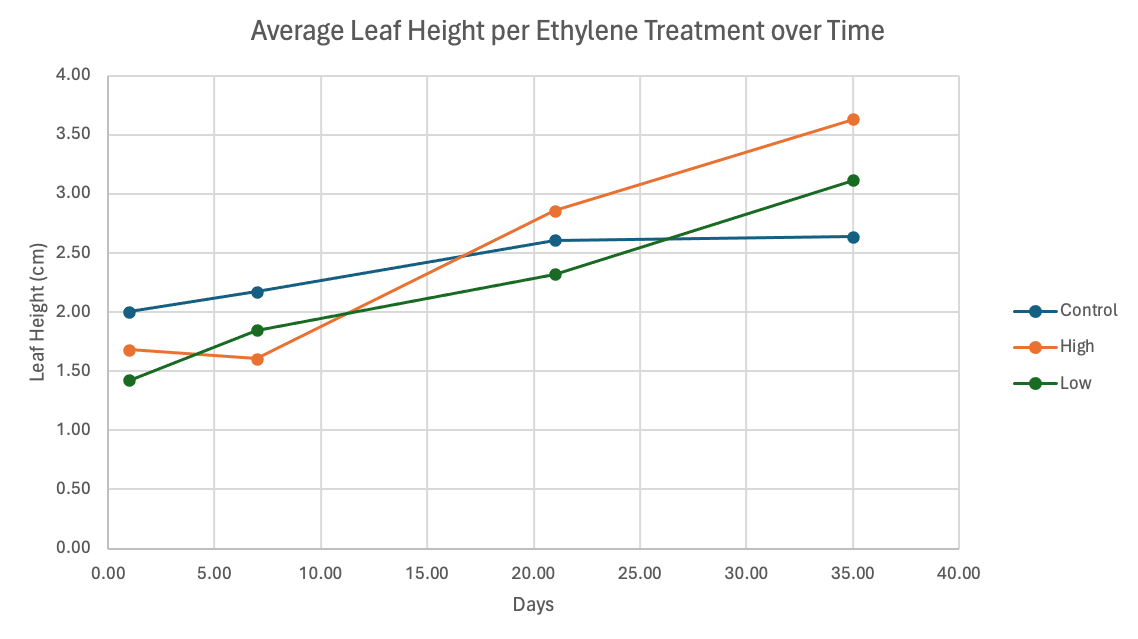
\includegraphics[width=\linewidth]{graph.png}
    \captionof{figure}{Average leaf height per ethylene treatment in \textit{Narcissus spp.} vegetation over time.}
  \end{Figure}
  \section*{Discussion}
  \lipsum[10]
  
\end{multicols}

\clearpage

\printbibliography

\end{document}